\documentclass[10pt,a4paper,twocolumn]{article}
\usepackage[margin=1.8cm,columnsep=0.7cm]{geometry}
\usepackage[T1]{fontenc}
\usepackage{lmodern,microtype}
\usepackage{amsmath,amssymb,bm}
\usepackage{graphicx,booktabs,multirow,xcolor}
\usepackage[hidelinks]{hyperref}
\usepackage[numbers,sort&compress]{natbib}
\usepackage{caption}
\usepackage{adjustbox}
\usepackage[section]{placeins}
\captionsetup{font=small,labelfont=bf}
\graphicspath{{figures/}}
\newcommand{\R}{\mathbb{R}}
\newcommand{\ov}{\operatorname{ov}}
\newcommand{\ControlParallax}{0.02}
\newcommand{\ControlSNR}{1.24}
\newcommand{\ControlVerdict}{degenerate}
\newcommand{\DriftChained}{1.12}
\newcommand{\DriftDirect}{0.13}
\newcommand{\RaftSpeedup}{---}
\newcommand{\ScaleErrMax}{0.6}
\providecommand{\ScaleErrMax}{---}
\providecommand{\RaftSpeedup}{---}
\providecommand{\ControlSNR}{---}
\providecommand{\DriftChained}{---}
\providecommand{\DriftDirect}{---}


\title{\textbf{Single-Pass Drone Video to 3D on One GPU:\\Overlap-Band Keyframes, a Parallax Test for ``Is It 3D?'',\\Monocular Depth Priors and Gaussian Splatting}}
\author{Team SIH\_2D-to-3D\\\small Smart India Hackathon 2026 --- Problem Statement 26158 (NTRO)}
\date{}

\begin{document}
\maketitle

\begin{abstract}
We present an end-to-end system that turns a single drone pass --- one video, no flight planning, no ground control --- into a 3D Gaussian Splatting model, a textured mesh and, when a flight log is available, georeferenced metric outputs. Every stage runs on one GPU: hardware video decoding, a keyframe selector built on dense optical flow, GPU structure from motion, a diffusion-transformer depth prior and splat training. The selector formalises the intuition that consecutive views must be \emph{similar enough to match and different enough to triangulate}: it chains optical flow to measure co-visibility and picks the sharpest frame inside an overlap band $[\tau,\tau+\delta]$, so every surface point is seen by about $1/(1-\tau)$ keyframes. Before any reconstruction it answers whether a pass contains recoverable 3D structure at all, using rotation-compensated parallax measured with \emph{direct} keyframe-pair flow and normalised by an estimated noise floor; chained tracks are unsuitable because their error grows linearly with the gap and masquerades as parallax. On edited 4K footage the selector finds the individual camera moves, and the keyframes it chooses all register. On a straight single-pass track we show that the usual 7-DoF GPS alignment silently rolls the model about the flight axis; levelling on the ground plane and fitting four degrees of freedom removes the failure and keeps metric scale error below \ScaleErrMax\% in simulation. All numbers are produced by scripts in the repository from the run directories.
\end{abstract}

\section{Introduction}
Operational mapping --- disaster response, inspection, reconnaissance --- often has one chance to fly over a site. Classical photogrammetry assumes the opposite: planned grids, high overlap, several passes and ground control points. Problem statement 26158 asks for an accurate, textured, georeferenced 3D model from \emph{a single pass} of a moving UAV~\cite{sih2026ps26158}.

A single pass is hard for three distinct reasons, and each one maps to a component of our system.
\begin{enumerate}
\item \textbf{Which frames?} A video carries thousands of highly redundant frames and a few bad ones (motion blur, compression, fades). Sampling at a fixed rate is the common default; it either wastes compute or, where the drone moves fast, leaves gaps that break the reconstruction into pieces (\S\ref{sec:keyframes}).
\item \textbf{Is it 3D at all?} A drone that yaws on the spot, or looks at a distant or planar scene, produces video in which a homography explains every frame pair. No amount of computation recovers depth from such footage; the system should say so before spending it (\S\ref{sec:verdict}).
\item \textbf{Where is it?} A single pass is nearly a straight line. Aligning the model to GPS through camera centres alone leaves the roll about that line undetermined (\S\ref{sec:georef}).
\end{enumerate}
Around these we assemble a GPU pipeline: NVDEC decoding, RAFT optical flow~\cite{teed2020raft}, spirula-studio's GPU structure from motion and 3D Gaussian Splatting~\cite{spirulastudio,kerbl2023gaussians}, and the Marigold~v2 depth prior~\cite{pavlovic2026marigoldv2} aligned to, and scored against, the SfM points.

\paragraph{Contributions.}
(i) An overlap-band keyframe selector over chained dense flow with an explicit multiplicity model, and pass segmentation for edited footage.
(ii) A per-pass 3D verdict from direct-flow residual parallax with a data-driven noise floor, validated on a synthetic pure-rotation control; we report where Torr's GRIC~\cite{torr1998gric} fails on flow correspondences.
(iii) A measurement of chained versus direct optical-flow correspondence error against exact ground truth.
(iv) A ground-levelled 4-DoF georeferencing rule with a significance test for sloped terrain, leave-one-out error and a jackknife scale uncertainty.
(v) An engineering study of keeping an A100 busy: removing host synchronisation from RAFT, CUDA-Graph replay, GPU colour conversion and nvJPEG/NVENC, with utilisation recorded for every stage.

\section{Related work}
\paragraph{Structure from motion and splatting.}
Incremental SfM as in COLMAP~\cite{schoenberger2016sfm} remains the reference for camera recovery; spirula-studio re-implements an incremental mapper on the GPU and adds sequence-aware matching for video~\cite{spirulastudio}. 3D Gaussian Splatting~\cite{kerbl2023gaussians} represents a scene as anisotropic Gaussians optimised by differentiable rasterisation; gsplat~\cite{ye2025gsplat} provides the rasteriser we use for fly-through rendering.
\paragraph{Keyframe selection.}
Visual SLAM systems insert keyframes by co-visibility and tracking quality, and ORB-SLAM chooses between homography and fundamental-matrix initialisation by model scores~\cite{murartal2015orbslam}; Torr's GRIC formalises that choice~\cite{torr1998gric}. We use dense flow with the forward--backward consistency test of Sundaram et al.~\cite{sundaram2010tracks}.
\paragraph{Monocular depth.}
Marigold~\cite{ke2024marigold} repurposed a latent diffusion model for affine-invariant depth; Marigold~v2~\cite{pavlovic2026marigoldv2} fine-tunes the Qwen-Image-Edit diffusion transformer~\cite{wu2025qwenimage} to predict affine-invariant log depth in one step. Depth Anything~V2~\cite{yang2024dav2} is a strong discriminative alternative.
\paragraph{Compositional reconstruction.}
WorldSculpt~\cite{niu2026worldsculpt} lifts per-object priors into cluttered scenes from posed, masked views; we discuss it as a downstream extension in \S\ref{sec:limits}.

\section{Method}
\begin{figure*}[t]
\centering
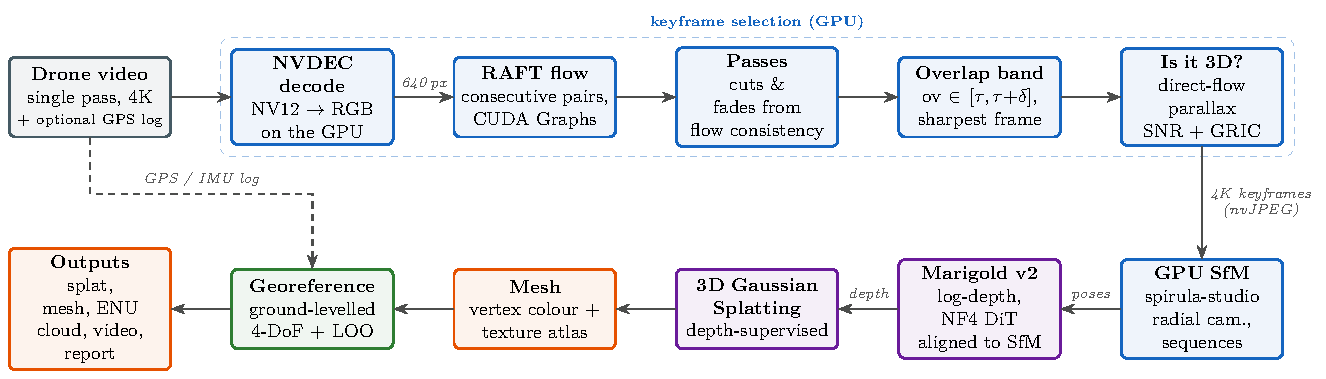
\includegraphics[width=\textwidth]{pipeline.pdf}
\caption{Pipeline. Everything between the video and the outputs runs on one GPU; stages exchange files only, so any stage can be re-run alone.}
\label{fig:pipeline}
\end{figure*}

\subsection{GPU ingest}
Frames are decoded by NVDEC through ffmpeg (\texttt{-hwaccel cuda}), resized on the GPU (\texttt{scale\_cuda}) and leave the decoder as raw NV12; conversion to RGB (BT.709, limited range) runs in PyTorch on the GPU. A background thread streams chunks so decoding overlaps optical flow. Keyframes are later re-decoded at full resolution, selected by timestamp in groups of 48 on concurrent decoder sessions, and encoded with nvJPEG. Frame indices of the analysis and extraction passes agree exactly (\S\ref{sec:exp}).

\subsection{Pass segmentation}
For analysis frames $I_0,\dots,I_{N-1}$ (long side 640\,px, $\approx$12\,fps) we compute RAFT flow $\mathbf{f}_t$ from $t$ to $t{+}1$ and $\mathbf{b}_t$ back, and the share $c_t$ of pixels passing the forward--backward test $\lVert\mathbf{f}+\mathbf{b}\rVert^2 < 0.01(\lVert\mathbf{f}\rVert^2+\lVert\mathbf{b}\rVert^2)+0.5$~\cite{sundaram2010tracks}. Inside a continuous camera move $c_t$ stays high; a cut, fade or dissolve collapses it. A \emph{pass} is a maximal run with $c_t \ge 0.35$, no dark or flat frame, and at least 2\,s; its ends are trimmed while they are darker than $0.8\times$ the pass median, removing fade-ins and fade-outs (a fade kills tracks, so without trimming it attracts keyframes, and a fade frame is a meaningless held-out view). Letterbox bars are found before analysis from the per-row and per-column maximum luma over twelve seek-sampled frames and cropped on the GPU: static black would otherwise count as perfectly tracked content, inflating overlap, and as trivially correct pixels, inflating held-out PSNR. Real footage is often edited; a true single pass yields one pass, and SfM rejoins passes that turn out to share views.

\subsection{Overlap-band keyframes}\label{sec:keyframes}
A grid $G$ of points (8\,px spacing) on keyframe $K$ is chained through the consecutive flows; a track dies when it fails the consistency test or leaves the frame. With $A_t\subseteq G$ the tracks alive at frame $t$,
\begin{equation}
\ov(K,t) = \min\Big(\tfrac{|A_t|}{|G|},\; \tfrac{|\mathcal{C}(A_t)|}{|\mathcal{C}|}\Big),
\end{equation}
where $\mathcal{C}$ are the 32\,px cells of frame $t$ and $\mathcal{C}(A_t)$ those containing a live track. The first term falls as $K$'s content leaves the view (forward motion), the second as new content enters it (backward motion), so the measure is symmetric in effect. The next keyframe is the sharpest frame (Laplacian variance relative to a 2\,s rolling median) among those with $\tau\le\ov(K,t)\le\tau+\delta$ before the curve first drops below $\tau$; defaults $\tau=0.75$, $\delta=0.1$. If the overlap drops below $\tau$ within one step, the next frame is taken to keep the chain connected.

\paragraph{Multiplicity.} Under uniform motion a point stays in view for about $1/(1-\tau)$ keyframe spacings, so each surface point is observed by $m\approx 1/(1-\tau)$ keyframes ($m=4$ at $\tau=0.75$) --- the ``two or more frames with a proper threshold of similarity'' that triangulation needs, stated as a design parameter. We report the measured multiplicity, $1+2\bar L$ with $\bar L$ the mean forward track length in keyframes.

\paragraph{Cost.} Only consecutive pairs are flowed, so analysis is linear in video length. An overlap matrix $M_{i,d}=\ov(i,i{+}d)$ for all frames and $d\le d_{\max}$ is built in one sweep: a fresh grid starts at every frame and all live grids advance together in a ring of $d_{\max}$ slots, one batched \texttt{grid\_sample} per frame and a single read-back; selection is then a CPU walk over $M$.

\subsection{Is it 3D? A parallax test}\label{sec:verdict}
For each keyframe $i$ we take its widest partner $j\le i+6$ with $\ov\ge0.3$, compute RAFT flow \emph{directly} between $I_{K_i}$ and $I_{K_j}$ in both directions, and keep consistent grid correspondences $(\mathbf{x}_n,\mathbf{y}_n)$. On a batch of all pairs we fit, by normalised DLT~\cite{hartley1997eightpoint} with Cauchy IRLS, a homography $H$ and a rank-2 fundamental matrix $F$. The residual $\lVert\mathbf{y}-H\mathbf{x}\rVert$ is rotation-compensated parallax: zero for pure rotation or a planar scene, growing with depth variation times baseline. We estimate the per-coordinate noise $\hat\sigma = 1.4826\,\operatorname{median}\sqrt{e_F^2}$ from $F$'s Sampson residuals $e_F$ --- pure noise whenever $F$ is correct, which includes degenerate motion --- and normalise
\begin{equation}
\mathrm{SNR} = \frac{\operatorname{median}_n\lVert\mathbf{y}_n-H\mathbf{x}_n\rVert}{\sqrt{2}\sqrt{2\ln2}\;\hat\sigma},
\end{equation}
where the denominator is the median transfer residual that isotropic noise in both views leaves, so SNR$=1$ means no measurable parallax. A pass is \emph{3D} when its median SNR over keyframe pairs is at least 2 and GRIC~\cite{torr1998gric} (both models scored on geometric error with $\hat\sigma$) prefers $F$ on at least 60\% of pairs; \emph{degenerate} when the SNR is below 1.5 and its 90th percentile below 2.

\paragraph{Why direct flow.} Chaining consecutive flows makes long-range correspondence cheap but its error accumulates with a systematic per-step bias (\S\ref{sec:exp}, Fig.~\ref{fig:drift}); over a keyframe span the drift reaches the size of the parallax being measured and is correlated across points, which the extra freedom of $F$ partly absorbs. Direct flow keeps the error near 0.1\,px at the same gaps.

\subsection{Structure from motion}
Keyframes are written per pass (\texttt{images/pass\_$k$/}) and reconstructed by spirula-studio's GPU SfM with each pass declared a sequence, so neighbours are matched and trusted first, plus GPU pair selection for loop closure. We use a \emph{single-focal} radial camera per pass: drone cameras have square pixels, and with independent $f_x,f_y$ the weak geometry of forward or orbital motion let the two drift 10--20\% apart for no gain in reprojection error (\S\ref{sec:exp}). Separate passes of an edited video become separate models unless they share views.

\subsection{Monocular depth prior}
Marigold~v2~\cite{pavlovic2026marigoldv2} predicts, per keyframe, $p(\mathbf{u})$ with $\log d(\mathbf{u}) = a\,p(\mathbf{u})+b$ for unknown $a,b$. It runs as upstream: 4-bit NF4 base transformer (what its LoRA was trained on), rank-128 LoRA and fine-tuned VAE decoder, one rectified-flow step, bf16 autocast, at 1024\,px; the quantised base is cached so a load reads $\approx$11\,GB rather than re-quantising 39\,GB. For every registered image the SfM tie points give depths $z_n$ at pixels $\mathbf{u}_n$.

\paragraph{Affine is not enough at landscape scale.} A Cauchy-IRLS fit of $\log z_n = a\,p(\mathbf{u}_n)+b$ works well where the tie points span a narrow depth range, but on drone footage the prior \emph{compresses the far field}: on Jal Mahal it places the far shore at the depth of the palace and the mountain ridge barely beyond it (Fig.~\ref{fig:depth}), so a single slope cannot fit both. We therefore calibrate each image with a monotone map: medians of $\log z$ in quantile bins of $p$, made non-decreasing by weighted pool-adjacent-violators, linear with the affine slope outside the knots. It keeps the prediction's ordering and lets the mapping bend. Both calibrations are scored on \emph{held-out} tie points (5-fold cross-validation per image).

\paragraph{Where the prior saturates.} In a distant pass every tie point may sit where the prediction has saturated at its far end; the correlation between $p$ and $\log z$ is then near zero or negative. The robust fit returns a non-positive slope and the stage writes no depth map for that image, so training is not supervised with wrong geometry.

The calibrated linear depth supervises splat training through spirula's Pearson-correlation depth loss (weight 0.05); pixels beyond $3\times$ the 99th-percentile SfM depth are left unsupervised. Because that loss is affine-invariant in \emph{linear} depth, the calibration --- which only SfM can provide --- shapes the supervision itself, not merely its reporting.

\subsection{Gaussian splatting and meshing}
Each SfM model with at least 8 images trains a 3DGS model in spirula-studio (30k steps, half resolution, bilateral-grid exposure correction), with every 8th keyframe held out for evaluation; meshes are extracted from the trained splats with vertex colour and texture atlases.

\subsection{Georeferencing a straight pass}\label{sec:georef}
With GPS positions $\mathbf{g}_n$ (local ENU) for camera centres $\mathbf{c}_n$, the usual fit is the 7-DoF similarity of Umeyama~\cite{umeyama1991}. If the $\mathbf{c}_n$ are nearly collinear the rotation about the line is unobservable and GPS noise sets it; the in-sample RMSE still looks like GPS noise because the unobservable direction does not affect it. We instead estimate the model's ground normal $\mathbf{n}$ by RANSAC on the sparse points (oriented towards the cameras), rotate $\mathbf{n}$ to $+z$, and fit yaw, scale and translation --- scale and yaw by complex least squares on horizontal coordinates, the vertical offset as a mean residual. The full similarity is used only if the track spans two dimensions \emph{and} its tilt against $\mathbf{n}$ exceeds $5^\circ$ by three jackknife standard errors, i.e.\ GPS proves the ground is sloped. We report leave-one-out RMSE rather than in-sample RMSE, and a jackknife relative standard error of the scale as the scale check.

\subsection{Keeping the GPU busy}
Stock torchvision RAFT rebuilds its correlation lookup offsets on the CPU in each of its 12 refinement iterations, divides by a CPU tensor, builds coordinate grids on the CPU, and upsamples the flow after every iteration although inference keeps only the last; at 640\,px a call cost roughly the same whatever the batch size, a sign of launch- and sync-bound execution. Removing these (identical arithmetic, differences $\le$ bf16 noise) and replaying the network from a CUDA Graph raised throughput \RaftSpeedup-fold. The selector's tracking avoids boolean-mask indexing, whose \texttt{nonzero} forces a host sync, in favour of scatter and redirected writes. Every stage runs under an NVML sampler recording utilisation, power, memory and the presence of other processes on the GPU, so no timing is reported without its context.

\section{Experiments}\label{sec:exp}

\paragraph{Setup.} One NVIDIA A100 80\,GB PCIe, shared with other users' jobs throughout (each stage's record states the GPU's occupancy); PyTorch 2.14 with CUDA 13.2, Python 3.14, ffmpeg 9.0 (NVDEC/NVENC), spirula-studio 2026.9.24 (Vulkan backend). Data: fifteen public drone videos (Table~\ref{tab:data}); they carry no flight logs.

\begin{table}[htbp]
\centering\small
\caption{Sample footage (public YouTube re-encodes, VP9).}\label{tab:data}
\begin{adjustbox}{max width=\linewidth}
\begin{tabular}{lrrr}
\toprule
Video & Resolution & fps & s \\
\midrule
ANGKOR WAT Breathtaking  Cinemati & 3840$\times$2160 & 24.00 & 193 \\
Above clouds & 2560$\times$1440 & 50.00 & 115 \\
Aerial Views of Rural Riches & 2560$\times$1440 & 23.98 & 19 \\
Breathtaking Aerial Views of Hanoi & 3840$\times$2160 & 29.97 & 103 \\
Colosseum like never before & 3840$\times$2160 & 29.97 & 135 \\
Eiffel Tower Drone 4k & 3840$\times$2160 & 29.97 & 306 \\
FPV Drone Flight through Beautiful & 3840$\times$2160 & 30.00 & 67 \\
GoPro & 1080$\times$1920 & 29.97 & 18 \\
HAGIA SOPHIA 4K & 3840$\times$2160 & 29.97 & 85 \\
Jal Mahal, Jaipur, India, Drone Ci & 3840$\times$2160 & 24.00 & 55 \\
Notre Dame Drone Paris 4k & 3840$\times$2160 & 29.97 & 214 \\
Petronas Twin Tower in FPV drone & 3840$\times$2160 & 59.94 & 35 \\
Qutub Minar, New Delhi, India 4K D & 3840$\times$2160 & 29.97 & 187 \\
Reichstag Berlin  in 4K & 3840$\times$2160 & 30.00 & 130 \\
The Messiah & 3840$\times$2160 & 29.97 & 94 \\
\bottomrule
\end{tabular}
\end{adjustbox}
\end{table}

\subsection{Passes, keyframes and the 3D verdict}

\begin{table*}[htbp]
\centering\small
\caption{Pass segmentation and keyframes per run. Overlap: mean co-visibility with the previous keyframe; views: measured views per point; SNR: median direct-flow parallax SNR (1 = none).}\label{tab:keyframes}
\begin{adjustbox}{max width=\linewidth}
\begin{tabular}{llrrrrrl}
\toprule
Run & Pass & Time (s) & KF & Overlap & Views & SNR & Verdict \\
\midrule
jal\_mahal & 0 & 0.0--7.4 & 30 & 0.77 & 6.9 & 22.4 & 3d \\
jal\_mahal & 1 & 8.0--14.1 & 14 & 0.79 & 5.2 & 3.6 & 3d \\
jal\_mahal & 2 & 14.2--23.8 & 59 & 0.77 & 7.7 & 6.0 & 3d \\
jal\_mahal & 3 & 23.8--36.0 & 97 & 0.74 & 7.4 & 16.3 & 3d \\
jal\_mahal & 4 & 37.2--54.0 & 13 & 0.86 & 8.2 & 3.2 & 3d \\
\bottomrule
\end{tabular}
\end{adjustbox}
\end{table*}

On Jal Mahal the flow signal splits the edit into 5 passes at its cuts and fades, and the band selects 213 keyframes; the mean overlap with the previous keyframe lies in 0.74--0.86, inside or just above the target band, and every pass is judged \emph{3d} (Table~\ref{tab:keyframes}). Decoding and flow for the 658 analysis frames took 37\,s, selection 12\,s and 4K extraction 45\,s.

\paragraph{Negative control.} A synthetic clip of a camera rotating about its centre over one real 4K frame (\texttt{tools/make\_degenerate\_clip.py}) has no parallax by construction. It yields SNR 1.24 (median residual 0.02$^\circ$) and the verdict \emph{degenerate}; GRIC nonetheless preferred $F$ on 60\% of its pairs, which is why GRIC only confirms the SNR decision.

\begin{figure}[t]\centering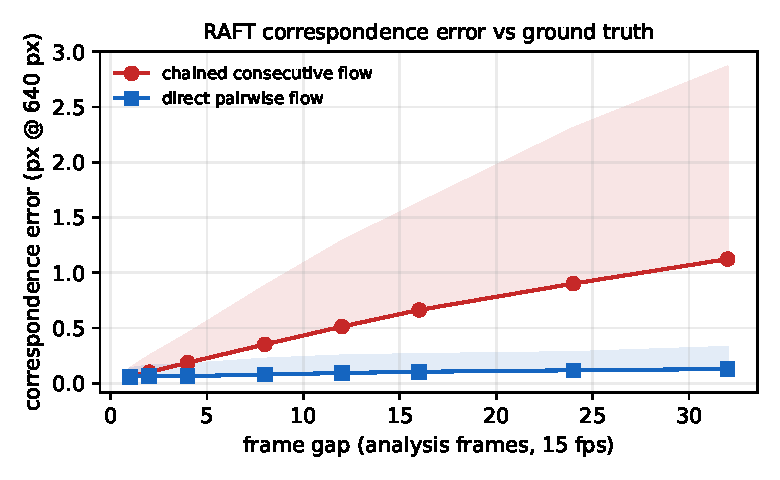
\includegraphics[width=\linewidth]{flow_drift.pdf}\caption{Correspondence error against exact ground truth on the rotation control. Chained consecutive flow drifts almost linearly (1.12\,px median at 32 frames); direct pairwise flow stays at 0.13\,px.}\label{fig:drift}\end{figure}

\subsection{Structure from motion}

With the same SfM settings, 1\,fps sampling registers 40 of 55 frames in 2 disconnected models (the largest 22), and uniform sampling at the selector's budget of 241 frames registers 237 but splits into 4 models (largest 98). The overlap band registers all 241 (largest 155); after cropping the letterbox and trimming fades the canonical run registers 213 of 213 (Table~\ref{tab:sampling}). A model per group of passes is expected: the passes of a cinematic edit are cut from different flights and need not overlap. One focal length per pass keeps the reprojection error while OpenCV's independent $f_x,f_y$ drift apart (Table~\ref{tab:camera}).

\begin{table}[htbp]
\centering\small
\caption{Structure from motion on the selected keyframes.}\label{tab:sfm}
\begin{adjustbox}{max width=\linewidth}
\begin{tabular}{lrrrrr}
\toprule
Run & KF & Registered & Models & Reproj. (px) & Time (s) \\
\midrule
jal\_mahal & 213 & 213 & 4 & 0.79 & 255 \\
\bottomrule
\end{tabular}
\end{adjustbox}
\end{table}

\begin{table}[htbp]
\centering\small
\caption{Frame sampling on Jal Mahal (same SfM settings).}\label{tab:sampling}
\begin{adjustbox}{max width=\linewidth}
\begin{tabular}{lrrrrl}
\toprule
Sampling & Frames & Registered & Models & Largest &  \\
\midrule
1 fps (uniform) & 55 & 40 & 2 & 22 & no letterbox crop \\
uniform, same budget & 241 & 237 & 4 & 98 & no letterbox crop \\
overlap band (dev) & 241 & 241 & 4 & 155 & no letterbox crop \\
overlap band (canonical) & 213 & 213 & 4 & 156 & cropped, fades trimmed \\
\bottomrule
\end{tabular}
\end{adjustbox}
\end{table}

\begin{table}[htbp]
\centering\small
\caption{Camera model on Jal Mahal: independent $f_x,f_y$ (OpenCV) against one focal (radial).}\label{tab:camera}
\begin{adjustbox}{max width=\linewidth}
\begin{tabular}{llrr}
\toprule
Camera & Focal(s) per pass (px) & Reproj. (px) & Points \\
\midrule
OpenCV (fx, fy free) & 3112/2812, 2055/2080, 2827/3382, 2986/2754 & 0.761 & 96{,}940 \\
radial (one focal) & 3118, 2684, 2808, 3109 & 0.771 & 96{,}598 \\
\bottomrule
\end{tabular}
\end{adjustbox}
\end{table}

\subsection{Monocular depth prior}

Table~\ref{tab:depth} scores each calibration on tie points it was not fitted to. The monotone map lowers held-out AbsRel on every model with depth; the gain is largest where the scene spans a wide depth range (Fig.~\ref{fig:depth}), which a single log-affine map cannot follow. Model~3 (30 keyframes, the far lake-side pass) has no image whose prediction correlates positively with its tie-point depths; it is trained without depth rather than with a wrong one.

\begin{figure*}[t]\centering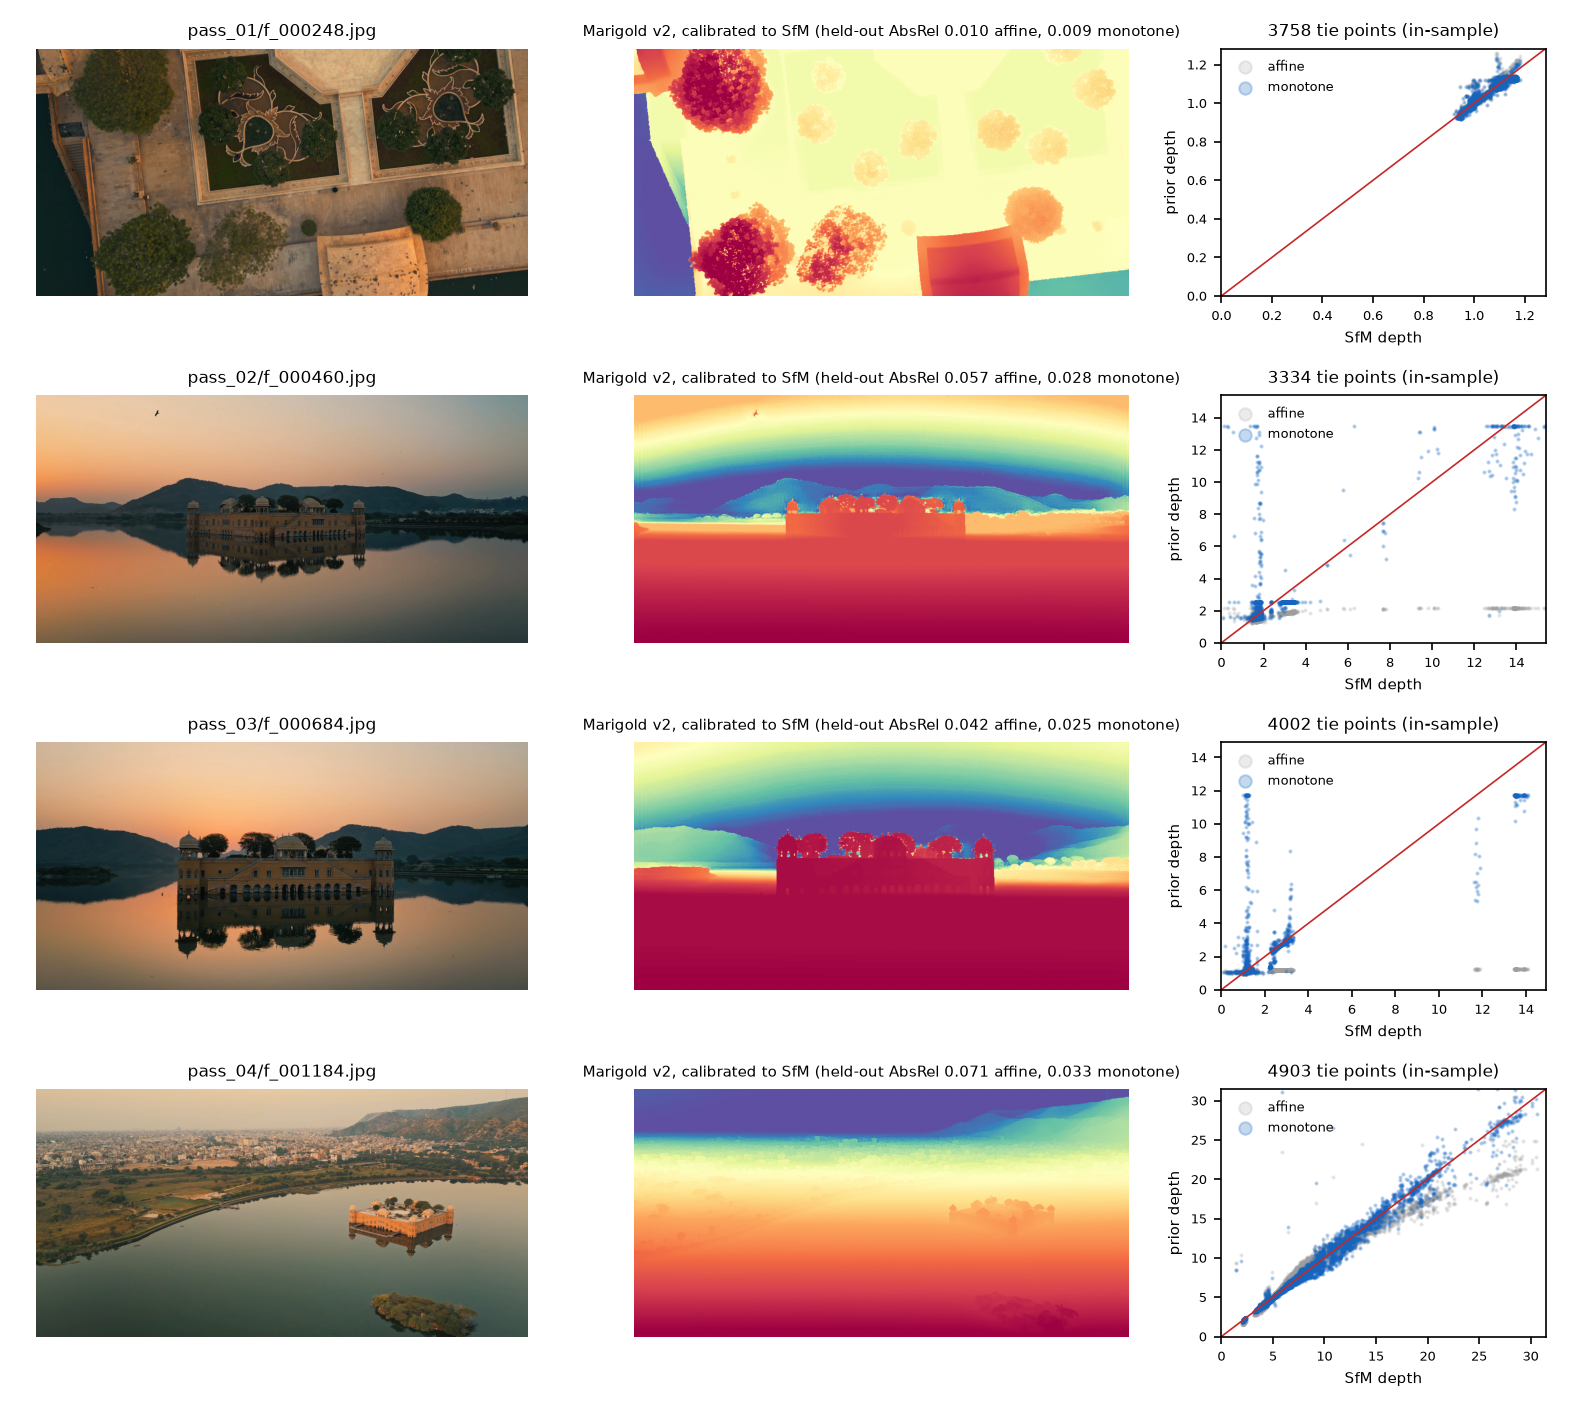
\includegraphics[width=0.92\textwidth]{depth_panel.png}\caption{Marigold~v2 on Jal Mahal keyframes (canonical run). Right: prior depth against SfM tie-point depth for the log-affine fit (grey) and the monotone calibration (blue). On the lake-facing passes the affine fit flattens the far shore and the ridge; the monotone map follows them (it also sends a few near points far). Held-out AbsRel for both is given above each depth map.}\label{fig:depth}\end{figure*}

\begin{table}[htbp]
\centering\small
\caption{Marigold~v2 against SfM tie points, scored on held-out tie points (5-fold cross-validation per image, median over images): log-affine vs monotone calibration.}\label{tab:depth}
\begin{adjustbox}{max width=\linewidth}
\begin{tabular}{llrrrrr}
\toprule
Run & Model & Aligned & AbsRel aff. & AbsRel mono. & $\delta_1$ aff. & $\delta_1$ mono. \\
\midrule
jal\_mahal & 0 & 156/156 & 0.050 & 0.027 & 0.857 & 0.886 \\
jal\_mahal & 1 & 14/14 & 0.009 & 0.006 & 1.000 & 1.000 \\
jal\_mahal & 2 & 13/13 & 0.075 & 0.033 & 0.945 & 0.989 \\
jal\_mahal & 3 & 0/30 & --- & --- & --- & --- \\
\bottomrule
\end{tabular}
\end{adjustbox}
\end{table}

\subsection{Gaussian splatting}

\begin{table*}[htbp]
\centering\small
\caption{3DGS on held-out keyframes (every 8th keyframe never used in training).}\label{tab:splat}
\begin{adjustbox}{max width=\linewidth}
\begin{tabular}{llrrrrr}
\toprule
Run & Model & Splats & PSNR & SSIM & LPIPS & Train (s) \\
\midrule
jal\_mahal & model\_0, depth prior (v1 mask) & 3{,}000{,}000 & 35.00 & 0.977 & --- & 3822 \\
\bottomrule
\end{tabular}
\end{adjustbox}
\end{table*}

\subsection{Georeferencing a straight pass}

None of the sample videos carries a flight log, so georeferencing is evaluated in simulation (\texttt{experiments/georef\_study.py}): a 300\,m track at 80\,m altitude over flat ground with buildings, the SfM model hidden behind a random similarity, horizontal GPS noise, and a sideways deviation of the track from a straight line of 0--60\,m; the error is measured at ground points 100\,m off the track. (Sloped ground, where the rule falls back to the similarity, is covered by the unit tests.) The levelled fit is never worse than the similarity (worst 2.1\,m) and its metric scale error stays below 0.6\,\% (Table~\ref{tab:georef}, Fig.~\ref{fig:georef}).

\begin{figure*}[t]\centering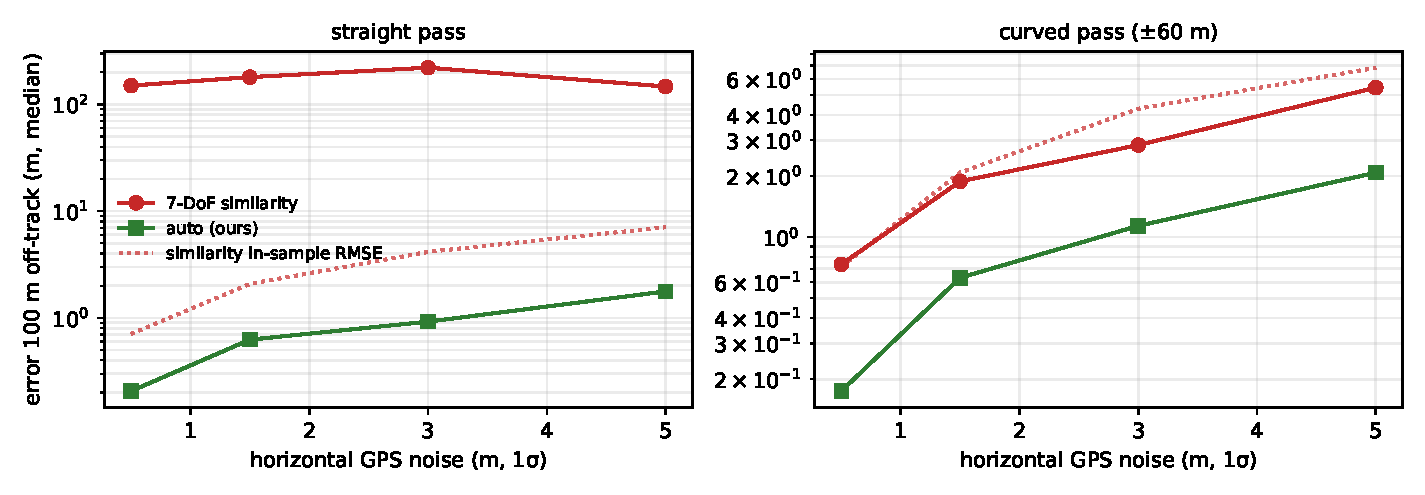
\includegraphics[width=0.85\textwidth]{georef_study.pdf}\caption{Error of ground 100\,m off-track after GPS alignment (median of 20 synthetic scenes per point). The 7-DoF similarity is off by up to 221\,m on a straight pass while its in-sample RMSE (dotted) only reflects GPS noise; the ground-levelled fit stays near the GPS noise.}\label{fig:georef}\end{figure*}

\begin{table*}[htbp]
\centering\small
\caption{Georeferencing study (medians over 20 trials): off-track error of the similarity and of our rule, in-sample RMSE of the similarity, held-out RMSE of ours, metric scale error.}\label{tab:georef}
\begin{adjustbox}{max width=\linewidth}
\begin{tabular}{rrrrrrr}
\toprule
GPS $\sigma$ (m) & Lateral (m) & Sim. (m) & Ours (m) & Sim. in-sample & Ours LOO & Scale err. \\
\midrule
0.5 & 0 & 149.9 & 0.21 & 0.71 & 0.73 & 0.1\% \\
0.5 & 5 & 5.5 & 0.19 & 0.69 & 0.71 & 0.0\% \\
0.5 & 20 & 2.1 & 0.19 & 0.68 & 0.70 & 0.0\% \\
0.5 & 60 & 0.7 & 0.17 & 0.72 & 0.74 & 0.1\% \\
1.5 & 0 & 180.0 & 0.62 & 2.08 & 2.16 & 0.1\% \\
1.5 & 5 & 19.5 & 0.54 & 2.10 & 2.18 & 0.1\% \\
1.5 & 20 & 5.0 & 0.58 & 2.16 & 2.24 & 0.2\% \\
1.5 & 60 & 1.9 & 0.63 & 2.08 & 2.16 & 0.2\% \\
3.0 & 0 & 220.7 & 0.92 & 4.15 & 4.29 & 0.2\% \\
3.0 & 5 & 27.0 & 1.11 & 4.00 & 4.15 & 0.2\% \\
3.0 & 20 & 7.6 & 1.29 & 4.28 & 4.44 & 0.3\% \\
3.0 & 60 & 2.8 & 1.14 & 4.29 & 4.44 & 0.2\% \\
5.0 & 0 & 146.9 & 1.77 & 7.08 & 7.32 & 0.3\% \\
5.0 & 5 & 24.4 & 2.13 & 7.13 & 7.37 & 0.5\% \\
5.0 & 20 & 11.0 & 1.59 & 6.92 & 7.14 & 0.4\% \\
5.0 & 60 & 5.4 & 2.08 & 6.83 & 7.07 & 0.6\% \\
\bottomrule
\end{tabular}
\end{adjustbox}
\end{table*}

\subsection{Throughput and GPU use}

\begin{table*}[htbp]
\centering\small
\caption{Per-stage wall time and GPU use (NVML, 0.5\,s samples). Own/host: peak GPU memory and host RSS of our process tree.}\label{tab:gpu}
\begin{adjustbox}{max width=\linewidth}
\begin{tabular}{llrrrrrl}
\toprule
Run & Stage & s & Util.\% & W & Own GPU (GB) & Host (GB) & Shared \\
\midrule
jal\_mahal & keyframes & 109 & 83 & 256 & 10.6 & 6.3 & yes \\
jal\_mahal & sfm & 256 & 83 & 213 & 9.9 & 4.2 & yes \\
jal\_mahal & depth & 522 & 84 & 265 & 24.3 & 11.2 & yes \\
\bottomrule
\end{tabular}
\end{adjustbox}
\end{table*}

\subsection{Fast profile: mesh and point cloud within the time budget}\label{sec:fast-results}

\paragraph{Structure from flow.} On the 97-keyframe orbit of Jal Mahal, tracks from direct RAFT flow register every keyframe; with 960\,px tracks the global mapper's camera centres agree with spirula's SIFT reconstruction to 0.19\,\% of the flight extent and its rotations to 0.28$^\circ$ (median), with no feature extraction or matching (Table~\ref{tab:flowsfm}). Tracking at 640\,px is cheaper but 2.5--3$\times$ less accurate. COLMAP's incremental mapper needs its initialisation angle lowered from 16$^\circ$ to 2$^\circ$ to start on single-pass footage at all and is eight times slower here.

\begin{table*}[htbp]
\centering\small
\caption{SfM from flow tracks on Jal Mahal pass 3 against SIFT SfM of the same keyframes (similarity-aligned).}\label{tab:flowsfm}
\begin{adjustbox}{max width=\linewidth}
\begin{tabular}{llrrrrrrr}
\toprule
Tracks & Mapper & Flow (s) & Map (s) & Reg. & Reproj. (px) & Centre (\% ext.) & Rot. med. ($^\circ$) & Rot. max ($^\circ$) \\
\midrule
640 px, 8 iterations & global & 8.8 & 9.8 & 97/97 & 0.32 & 0.53 & 0.79 & 1.44 \\
640 px, 12 iterations & global & 13.1 & 18.7 & 97/97 & 0.32 & 0.55 & 0.66 & 1.35 \\
960 px, 12 iterations & global & 28.9 & 16.2 & 97/97 & 0.32 & 0.19 & 0.28 & 0.41 \\
960 px, 12 iterations & incremental & 28.9 & 129.1 & 97/97 & 0.35 & 0.40 & 0.42 & 1.59 \\
\bottomrule
\end{tabular}
\end{adjustbox}
\par\smallskip\footnotesize Reference: spirula-studio SIFT SfM of all 213 Jal Mahal keyframes, 255\,s for extraction, matching and mapping.
\end{table*}

\paragraph{Fusion.} The depth maps (triangulated, then filled by the calibrated prior) cover every non-sky pixel of the references, yet a TSDF with the usual 4-voxel truncation band keeps only part of the view: neighbouring views disagree slightly and their signed distances cancel. Widening the band recovers most of it at a small cost in depth error against the triangulated geometry (Table~\ref{tab:tsdf}); the profile uses 12 voxels.

\begin{table}[htbp]
\centering\small
\caption{TSDF truncation band on Jal Mahal's two largest models (voxel = 3 pixel footprints at the median depth): view completeness, median depth error against the triangulated depth, triangles.}\label{tab:tsdf}
\begin{adjustbox}{max width=\linewidth}
\begin{tabular}{lrrrr}
\toprule
Model & Band (vox.) & Completeness & Depth err. (\%) & Triangles \\
\midrule
0 & 4 & 0.468 & 0.42 & 41{,}072 \\
0 & 8 & 0.722 & 0.51 & 184{,}092 \\
0 & 12 & 0.800 & 0.60 & 402{,}964 \\
0 & 16 & 0.853 & 0.68 & 666{,}407 \\
1 & 4 & 0.750 & 0.92 & 178{,}556 \\
1 & 8 & 0.874 & 1.05 & 416{,}504 \\
1 & 12 & 0.912 & 1.09 & 604{,}939 \\
1 & 16 & 0.928 & 1.10 & 743{,}658 \\
\bottomrule
\end{tabular}
\end{adjustbox}
\end{table}

\paragraph{Time and completeness.} The budget is 1.5$\times$ the video length (15 minutes for a 10-minute video). Completeness is the share of each registered keyframe's non-sky pixels whose ray hits the mesh. The motion-adaptive analysis rate costs a few points of completeness and brings the 187\,s Qutub Minar video within budget (243\,s of 281\,s); the 55\,s Jal Mahal edit, five camera moves over a lake, stays over it (147\,s of 82\,s). Measuring overlap against the points that survive the first tracking step (so that water does not force a keyframe every step) was worse on both videos (Table~\ref{tab:fastruns}).

\begin{table*}[htbp]
\centering\small
\caption{Fast profile end to end on a shared A100: keyframes, registration, view completeness, processing time and budget (1.5$\times$ video length). The adopted setting is the adaptive rate with absolute overlap.}\label{tab:fastruns}
\begin{adjustbox}{max width=\linewidth}
\begin{tabular}{lllrrrrr}
\toprule
Video & Analysis & Overlap & KF & Reg. & Compl. & Time (s) & Budget (s) \\
\midrule
Jal Mahal & 12 fps & absolute & 213 & 213 & 0.82 & 262 & 82 \\
Jal Mahal & adaptive, 3.0 fps & absolute & 128 & 128 & 0.78 & 147 & 82 \\
Jal Mahal & adaptive, 6.0 fps & relative & 82 & 82 & 0.71 & 145 & 82 \\
Qutub Minar & 15 fps & absolute & 110 & 102 & 0.81 & 307 & 281 \\
Qutub Minar & adaptive, 3.3 fps & absolute & 113 & 106 & 0.75 & 243 & 281 \checkmark \\
Qutub Minar & adaptive, 7.5 fps & relative & 106 & 98 & 0.70 & 292 & 281 \\
\bottomrule
\end{tabular}
\end{adjustbox}
\end{table*}

\paragraph{Georeferencing, end to end.} Each Jal Mahal model receives a known model-to-world similarity at the real site and its keyframes GPS with 1.5\,m horizontal and 3.0\,m vertical noise; the pipeline's georef and export stages then run unchanged. The levelled fit recovers rotation to a few tenths of a degree and scale to half a percent; the exported mesh is within 0.43--2.06\,m (median) of the truth within 100\,m of the track, and the error grows with distance, as yaw and scale error do (Table~\ref{tab:geoe2e}). LAS and GeoTIFF outputs carry EPSG:32643 (UTM 43N).

\begin{table*}[htbp]
\centering\small
\caption{Georeferencing with synthetic GPS on the real models: rotation error, scale error, held-out horizontal RMSE of the cameras, and median mesh error by distance from the flight track.}\label{tab:geoe2e}
\begin{adjustbox}{max width=\linewidth}
\begin{tabular}{llrrrrrr}
\toprule
Model & Fit & Rot. ($^\circ$) & Scale (\%) & LOO (m) & $<$100\,m & 100--300\,m & $>$300\,m \\
\midrule
0 & yaw-scale & 0.01 & 0.35 & 1.93 & 2.06 & 2.46 & 7.3 \\
1 & yaw-scale & 0.23 & 0.07 & 1.99 & 0.86 & 1.19 & 8.7 \\
2 & yaw-scale & 0.36 & 0.44 & 1.86 & --- & 2.53 & 68.8 \\
3 & yaw-scale & 0.02 & 0.47 & 2.11 & 0.43 & 0.72 & --- \\
4 & yaw-scale & 0.34 & 0.50 & 2.74 & --- & --- & 17.8 \\
5 & yaw-scale & 0.06 & 0.50 & 1.97 & --- & --- & --- \\
\bottomrule
\end{tabular}
\end{adjustbox}
\end{table*}


\FloatBarrier
\section{Limitations}\label{sec:limits}
\textbf{No flight logs in the public samples.} The fifteen sample videos are YouTube re-encodes without GPS; georeferencing is therefore evaluated in simulation (\S\ref{sec:exp}), and the georef stage runs on real data only when a DJI SRT, CSV, GPX or JSON log is supplied. \textbf{Edited footage.} The samples are edits of several shots; each pass becomes its own model, which a true single pass would not need. \textbf{Water and sky.} Reflections are reconstructed as mirrored geometry below the surface, as 3DGS always does, and single-frame flow-consistency dips on water add keyframes. \textbf{Shared GPU.} Timings were taken while other users' jobs shared the A100; each stage's record says so. \textbf{Compositional objects.} WorldSculpt~\cite{niu2026worldsculpt} could turn the splat scene into per-object meshes given instance masks and boxes; we have not integrated it.

\section{Conclusion}
A single drone pass can be turned into a splat model and mesh on one GPU in minutes, provided the system chooses its frames by what they see rather than by the clock, checks that the motion contains parallax before trusting it, and aligns to GPS with the constraint a straight line cannot provide. The code, configurations and the scripts that regenerate every number in this paper are in the repository.

\bibliographystyle{unsrtnat}
\bibliography{refs}
\end{document}
